\documentclass{sig-alternate-05-2015}
\usepackage{float}
\usepackage{hyperref}
\usepackage{subcaption}
\usepackage{booktabs}
\usepackage{algorithm}
\usepackage{algorithmic}


\begin{document}

% Copyright
%\setcopyright{acmcopyright}
% DOI

% ISBN

\title{Micro Cloud Platform for Processing Big Data in Bioinformatics}

\numberofauthors{1}
\author{
% 1st. author
\alignauthor
Brendan D. Ball\\
       \affaddr{University of Cape Town}\\
}

\date{30 August 2015}
\toappear{
The source code for the micro cloud platform is available as a git repository at \url{https://github.com/wraithy/bigbinf} in the cloud branch.\\
The NCBI NR database used in this paper is available at \url{ftp://ftp.ncbi.nlm.nih.gov/blast/db/} which takes 36GB of storage space. \\
The Blast search tool is available at \url{ftp://ftp.ncbi.nlm.nih.gov/blast/executables/blast+/LATEST}.\\
}


\maketitle
\begin{abstract}
Processing Big Data in Bioinformatics is often made difficult by the need to download the entire data set. The solution proposed is to create a micro cloud platform which would be deployed at various institutions. This micro cloud should allow users to process data without having to download it. Results are normally miniscule in size compared to the raw data, which makes them easy to download. A community cloud is formed by connecting micro clouds using a discovery service. A proof of concept is implemented and evaluated using sample Bioinformatics analysis code.
\end{abstract}
\keywords{Big Data; BioInformatics; Clouds}


\section{Introduction}
Cloud infrastructure is the combination of multiple compute and storage resources presented as a single system on the internet. Cloud computing has developed considerably over the last decade. Examples of commercial cloud offerings include Amazon Web Services and Google Compute Engine \cite{krishnan2015google, mathew2014overview}. Cloud infrastructure has the potential to simplify the processing of big data sets, as well as collaboration between remote researchers. 
\\
\\
The first step in simplifying processing of big data sets is to minimize the need for transferring the data. This can be done by storing the data in a cloud and allow researchers access to process the data on the cloud, instead of downloading the data first before processing it. Minimizing the need for transfers of Big Data is important because limitations in current internet infrastructure makes collaboration difficult when Big Data is involved. 
\\
\\
A commercial cloud such as Amazon EC2, still has the problem of uploading big data sets to the cloud infrastructure \cite{baker2010next}. Micro clouds deployed on-site will overcome this challenge by keeping the data locally, while still reaping the benefits of a cloud platform. However, with different research institutions deploying their own micro clouds, cloud interoperability is required to allow researchers from different institutions to collaborate on the same data. Cloud interoperability creates a community cloud. A use-case of a specific community cloud  by Jimenez et al. \cite{jimenez2014deploying} contains core architectural properties needed for a successful community cloud. These properties include autonomy (where each micro cloud is be managed independently), security, self management of nodes, and scalability.
\\
\\
The traditional approach to creating a cloud platform allows users to run their own instances of operating systems (such as Amazon EC2) via virtualisation technology. This includes both hardware level emulation support and the software needed to manage the virtualisation. These virtualisation schemes use machine level virtualisation \cite{fink2014docker}. \\\\
A new method, known as containerization, provides much of the same functionality, with added benefits of lower resource usage and better performance. Containers are able to run native machine instructions whereas virtualisation emulates every machine instruction \cite{dua2014virtualization}. Containers are only useful when complete virtualisation is not needed, but allow for isolated application deployment and portability. The use of containers instead of virtual machines has only recently become popular. The growth in popularity has resulted in a number of systems being developed including Rancher and Kubernetes. 
\\\\
Both virtualisation and containerization requires every instance to be configured by installing necessary software packages. Configuration can be time consuming, particularly in the context of bioinformatics. Cloud BioLinux is part of a cloud solution which solves this issue \cite{krampis2012cloud}. This toolkit makes it easy to deploy virtual machines to a cloud platform with bioinformatics infrastructure pre-configured. It bundles specific packages used in next generation sequence analysis (which is the processing of DNA data), thereby decreasing configuration time and increasing maintainability. Instances of Cloud BioLinux have been tested on the Amazon EC2 cloud platform and on a private Eucalyptus cloud. Eucalyptus is open source cloud software that enables you to create your own private cloud.
\\\\
Another project compatible with both Amazon EC2 and Eucalyptus is CloudMan \cite{afgan2015building}. CloudMan is designed as a workbench which manages cloud resources. A workbench relies on a pre-configured environment on which to execute code. It aims to improve biomedical data anaylsis and fully integrates with the Galaxy framework, a biomedical research platform. This cloud solution does not provide a user configurable execution environment as it relies on Galaxy tools to perform analyses. 
\\\\
We aim to provide users with a configurable environment, taking advantage of open source cloud software and Linux containers to enable efficient processing of Big Data through the use of micro clouds. The aim is to build a micro cloud platform and form a community cloud which allows sharing of data and collaboration of users between multiple micro clouds. Users can access data and submit jobs to the micro cloud by interacting with a front end web interface. Evaluation is done by deploying two micro clouds at UWC. The functionality is evaluated by uploading sample code and executing it on data which already exists on the cloud.
\\\\
UCT and UWC are collaborators on this project. UWC provided valuable hardware resources enabling thorough evaluation in a real world setting.

\section{Background}
Docker is built on top of Linux containers and is the main technology that we are using to build the micro cloud. To build a micro cloud platform, a cluster manager is required. We look at OpenStack and Kubernetes as possible systems for a cluster manager.


\subsection{Docker}
Docker is an implementation of a Linux container management tool. Docker functions similarly to virtualisation. It uses an image to quickly launch a pre-configured isolated environment. The key difference is that containers directly use the Linux kernel on the host machine to run native instructions, whereas virtual machines emulate the entire operating system, including the kernel. Every virtual machine launches its own kernel and is not aware of the host kernel. This key difference make containers lightweight, allowing them to be launched in a fraction of time compared to launching a virtual machine \cite{joy2015performance}. 
\\\\
Docker builds on Linux containers by implementing an image format which makes use of an AUFS filesystem. This allows a docker image to be built up from a number of intermediate layers. Layers can be added or removed without affecting another layer in the image \cite{boettiger2014introduction}.
\\\\
The layered approach to creating a Docker image allows images to be built using a script called a Dockerfile. Defining an image with a script makes docker images much more portable and reproducible compared to an image from a running environment, as is the case with virtualisation \cite{boettiger2014introduction}.
\\\\
The Docker group also hosts a publicly available image repository for upload or download of available Docker images. These images provide full disclosure of its configuration via its Dockerfile. This provides great community support with images for specific use-cases. An example is CloudBioLinux which officially only provides virtual machine images, however third parties have uploaded Docker images of CloudBioLinux available for anyone to use.

\subsection{OpenStack}
Openstack is a full stack cloud platform which manages compute, storage, and networking resources. OpenStack can be used to orchestrate virtual machines and has recently been extended to support docker containers as well. OpenStack aims to be a complete cloud solution which has resulted in it being cluttered, with many-inter dependent components \cite{affetti2015adock}. The required functionality  from a cluster manager for this project is limited compared to everything that OpenStack provides. A simpler cluster manager, specifically designed for use with docker is better suited for this project.


\subsection{Kubernetes}
Kubernetes is a pure container manager specifically designed to orchestrate Docker containers. Kubernetes version 1 has recently been released. Kubernetes is easy to use and not cluttered and aims to solve a single problem of being a container manager \cite{googleborg}. 
\\\\
Google used Linux containers long before Docker was created. Google developed its own in-house container orchestration system called Borg. Google created Kubernetes after learning from mistakes made in the design of Borg. Borg was orginally designed as a monolithic system which makes it difficult to scale. Kubernetes is much more modular and is easy to deploy \cite{googleborg}.


\section{Design And Implementation}


Cloud infrastructure comprises one or more clusters. A cluster is a collection of servers (nodes). Data storage is also part of cloud infrastructure, but is typically separated from compute nodes and accessed over the network. Our platform consists of the following components: a web interface, a scheduler, an image builder and image repository, a cluster manager (the master node), multiple worker nodes, and a storage interface which allows reading from and writing to persistent storage. Figure \ref{fig:architecture} shows the connection between these components.
\\\\
The functionality of the platform is of primary concern, thus user interface design is not considered and is outside the scope of this project. 

\begin{figure}[h]
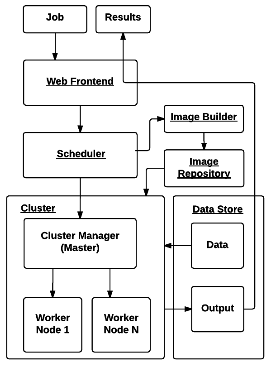
\includegraphics[width=8cm]{img/microcloud_architecture}
\caption{Our Micro Cloud Architecture showing the interaction between components of the cloud framework.}
\label{fig:architecture}
\end{figure}

\subsection{System Architecture}
Figure \ref{fig:architecture} gives an overview of how components interact. This section gives implementation-specific details for every component.

\subsubsection{Job}
A job describes a single instance of code uploaded for execution. 
The micro cloud platform Docker containers to execute code. Docker images are created with dockerfiles, which specify the execution environment and what files to execute. Submitting a job requires a Dockerfile and source code to be executed, uploaded together packaged as a single tar archive.  

\subsubsection{Cluster Manager}
To create a cloud platform with containers, a framework is needed to manage containers in a cluster which performs scheduling and resource allocation. OpenStack was the first system considered for use as a container manager. After much trouble setting up the development environment it was decided that there are more suitable systems to solve the problem. Kubernetes was chosen as the cluster manager framework for managing the micro cloud. 

\subsubsection{Image Builder}
A dedicated docker-in-docker container is run which is used to build docker images from dockerfiles. The image is then pushed to a private docker repository which can be accessed by any node in the cluster. The docker image is pulled by a worker node when the job is assigned to that worker node.

\subsubsection{Scheduler}
The default scheduler relies on first-in-first-out (FIFO) queues to schedule jobs. There are 3 FIFO queues: a build queue where dockerfiles are queued for the building process, a ready queue where Docker images are ready to be run, and an archiving queue where jobs are queued to have their results archived for downloading. The scheduler keeps track of running jobs using a list rather than a FIFO queue because running jobs are asynchronous. This means for example that job B can be started after job A and still still complete before job A. The number of concurrent jobs running is dependent on the number of worker nodes. Another two lists are used to keep track of completed jobs, one list for completed jobs with no results and another list for completed jobs with results ready to be downloaded. The completed jobs with no results queue is relevant because it is possible to directly interact with remote storage from within the container without using the cluster provided storage. An example of this is using object storage which is not suited for mounting as a filesystem.

\subsubsection{Storage}
The cluster at UWC makes use of Ceph storage which can be accessed by a RADOS Block Device (RBD). Kubernetes provides support for mounting an RBD as a storage volume in a container. However, due to difficulties getting Kubernetes to properly work with RBD during development, a different approach was taken. An RBD was mounted on the worker node outside of Kubernetes. It was then treated as a normal filesystem and mounted as host storage in the container. Using RBD in this way is still beneficial compared to using plain host storage as raw data doesn't have to be copied to each VM, which is infeasible given the size of most raw data in Bioinformatics (The raw data used during the evaluation of the system is 36GB).

\subsubsection{Web Interface}
The backend web interface is implemented using the Python flask web framework. It is a minimalist framework which allows for rapid development of web interfaces. 
The front end web interface is implemented using Angularjs to create a single page application. The website provides a form to submit a job by uploading a tar archive. Two text boxes are provided to allow the user to specify mount points (by means of an absolute file system path such as "/db" and "/results") for the raw data and results folder inside the container. Below the form is a list of jobs which shows each job's current status. This list is updated by polling the server every few seconds. If a job is complete and the results folder contains files then the user will be able to download the results as a tar archive. On a different web page (titled 'regions') is a list of all available micro clouds. The user can click on a region to navigate to a different micro cloud.

\subsubsection{Community Cloud}
A community cloud is formed by implementing a centralised discovery service. This improves scalability compared to a full mesh network between micro clouds. Figure \ref{fig:discovery} depicts how micro clouds are connected with the discovery service. The discovery service gives a list of connected micro clouds with their url (either an IP address or a domain) along with the name of the micro cloud. The discovery service has to be manually configured by adding a micro cloud's details to a configuration file.

\begin{figure}
\centering
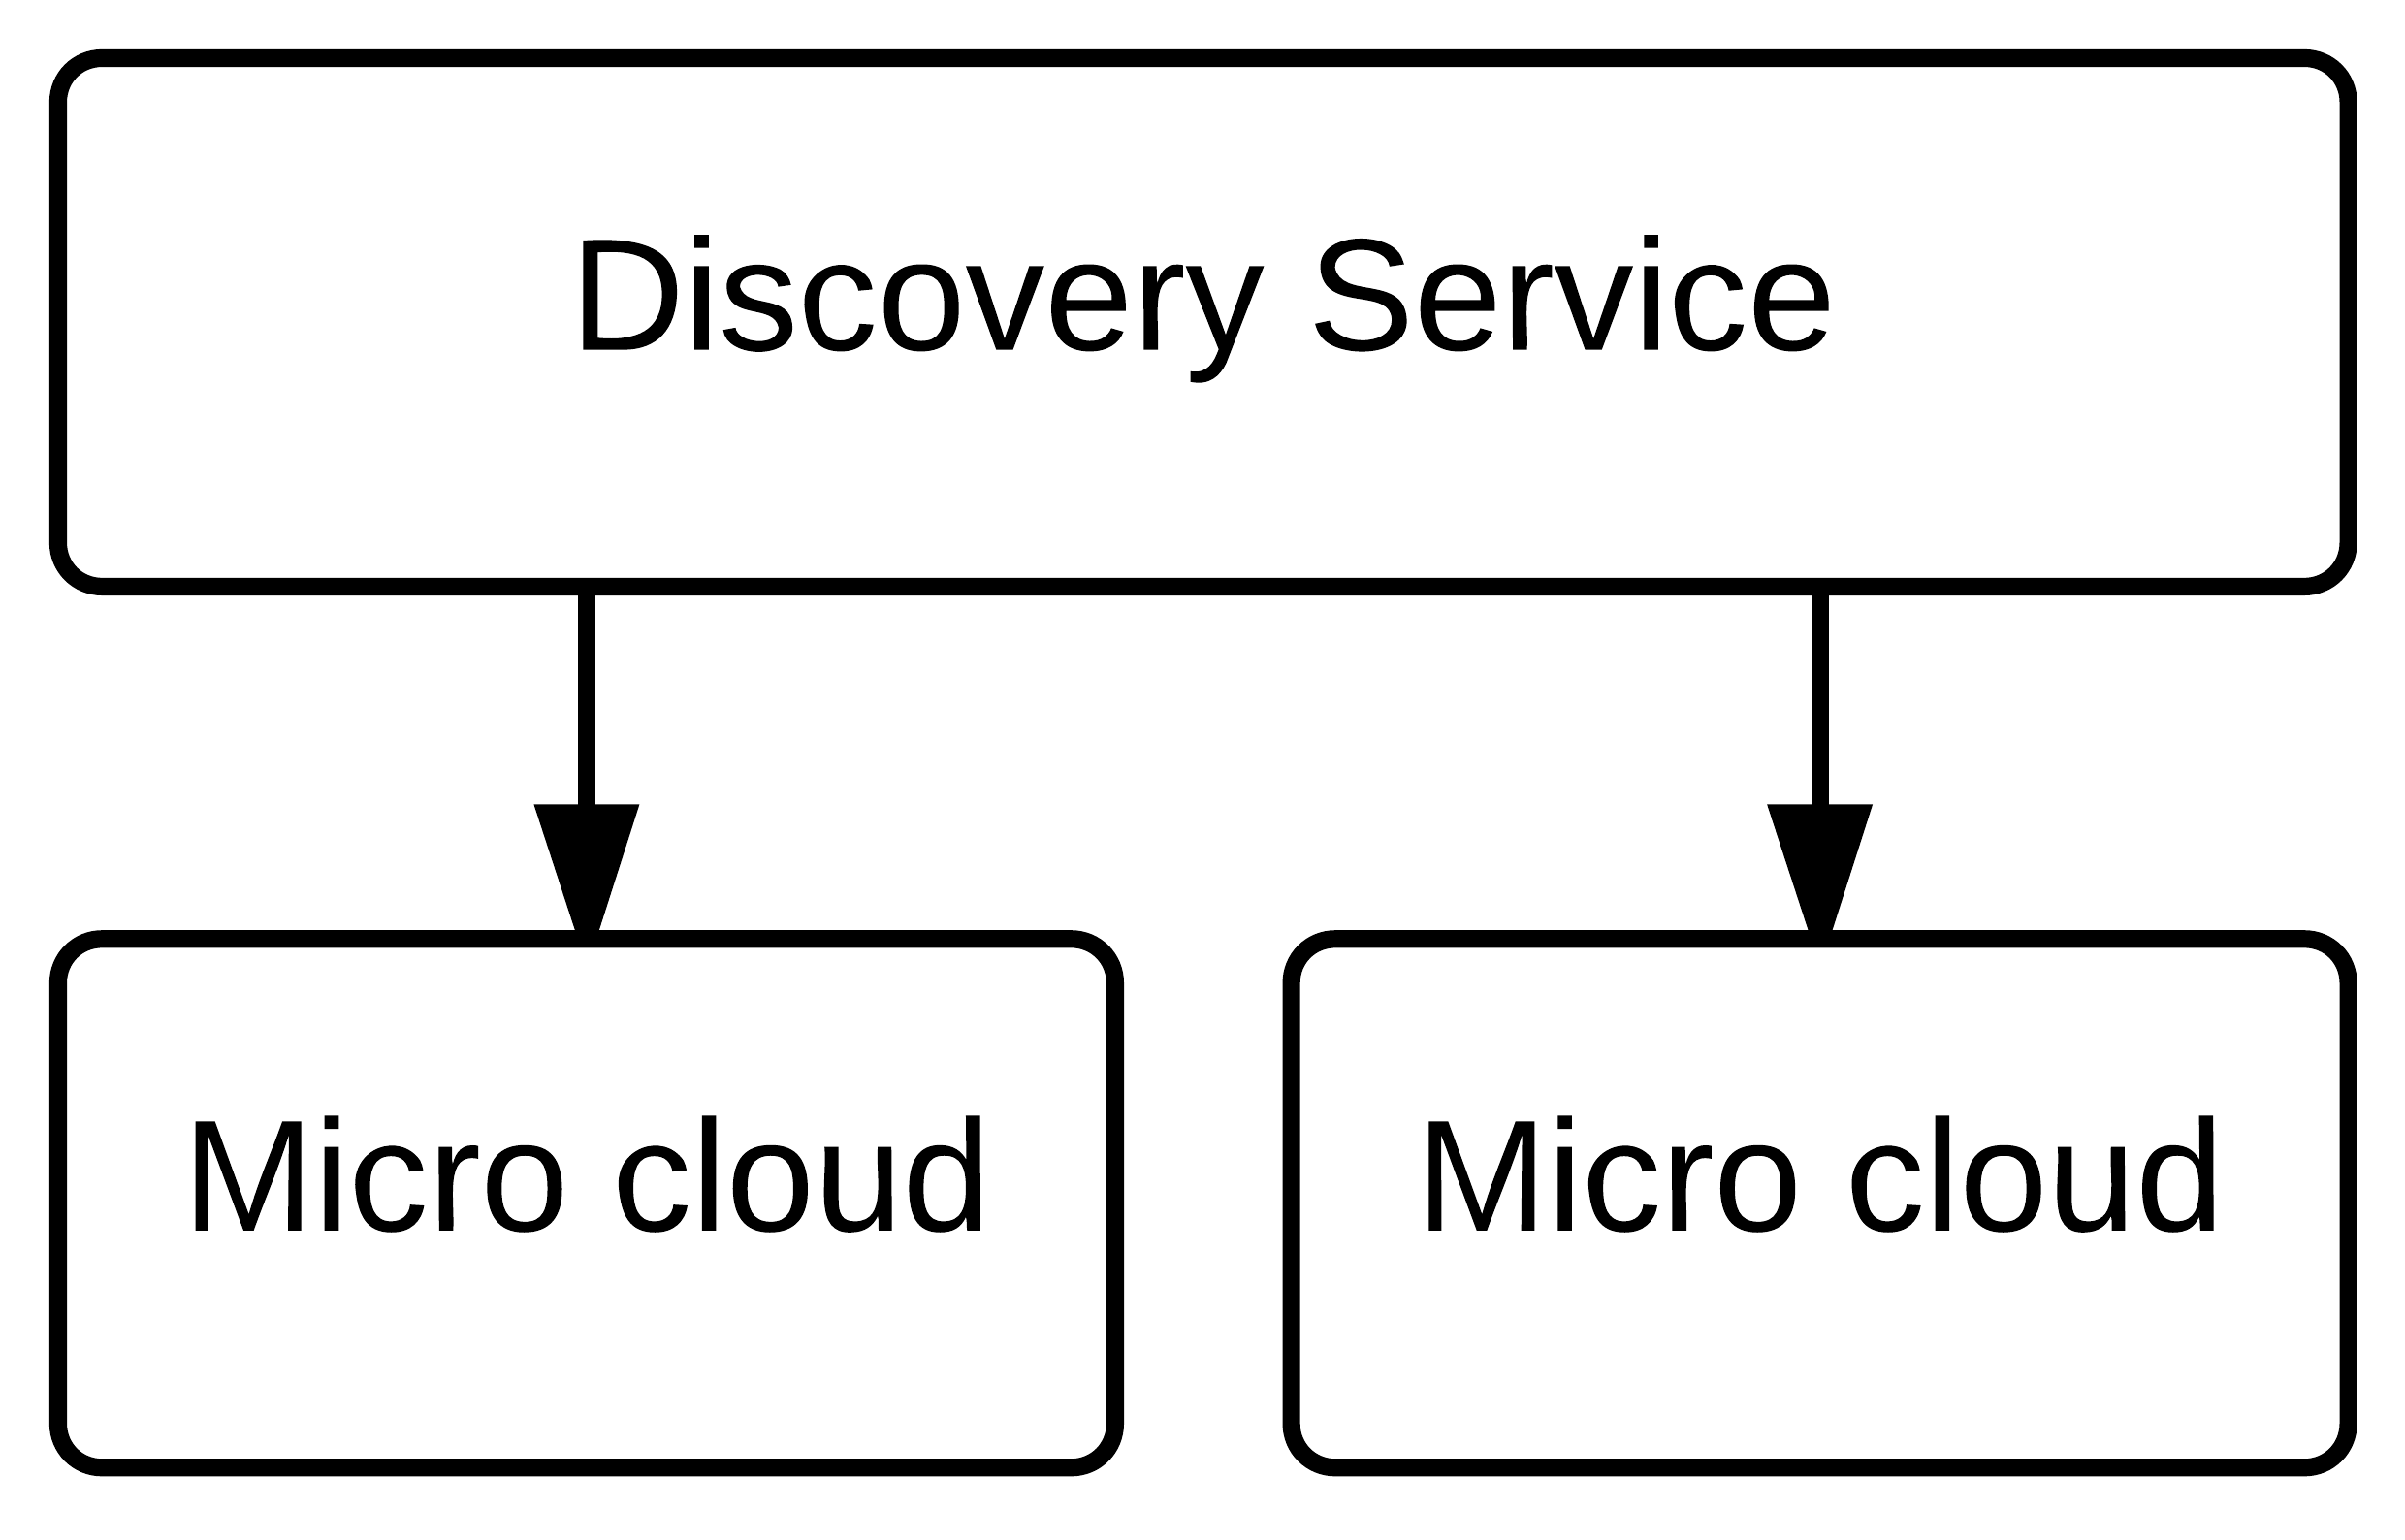
\includegraphics[scale=0.3]{img/communitycloud}
\caption{Community Cloud Architecture: Micro clouds are connected with a discovery service.}
\label{fig:discovery}
\end{figure}


\subsection{Constraints}
Micro cloud deployments for evaluation are limited to UWC. The evaluation was done on one community cloud containing two micro clouds. Each micro cloud was deployed on a single virtual machine (VM) as a single node cluster. Each VM has 1GB RAM, a single cpu, and 10GB of storage. Two 100Gb RBDs were provided, one for raw data and one for storing results. Due to both clusters residing on the same network, both clusters made use of the same storage. This would not be the case if each cluster was deployed at a different institution, but for the purposes of the evaluation it is not important.

\subsection{Software Engineering}

We implemented a proof-of-concept of the community cloud. The aim was not to focus on software engineering methodologies. However, to allow for reproducibility the source code is stored in a Git repository hosted on Github (Git is a version control system). All the components are containerized so a cluster can easily be deployed by running a few docker containers. This allows greater portability and reproducibility. 




\subsection{Evaluation}
The functionality of the micro cloud is evaluated by submitting sample Bioinformatics analysis code as a job. The analysis code searches against a genome database. We chose a database that is publicly hosted by the National Center for Biotechnology Information (NCBI), an institution dedicated to improving technologies used in genomic research \cite{pruitt2005ncbi}. The analysis code makes use of the Basic Local Alignment Search Tool (BLAST) \cite{camacho2009blast}. This tool specifies a database and submits a query containing specific search criteria. The job runs successfully if the container exits and results are available for download. The results consists of a single text file output by the BLAST tool which gives details according to the query submitted. Different sized jobs are tested by increasing or decreasing the size of the query, which makes it easily scalable to different sized test cases.
\\\\
The cloud platform was tested by submitting three jobs containing analysis code as described above. Each job tested a different sized query. After successful completion of each job the results were available for download, archived in a tar file. Each job's results contained a single text file created by the BLAST tool, which contained details about the query and the database and outputs generated based on evaluating the query with the database. The exact results output from the job do not give any insights regarding the evaluation of the cloud platform because we are testing the platform itself and not the analysis code. 


\section{Results and Discussion}
We have implemented the micro cloud proof-of-concept and evaluated it using Bioinformatics analysis code. Figure \ref{fig:screenshots} shows the web interface available to the user. 

\subsection{Submit a Job}
Figure \ref{fig:screenshot2} shows the form for submitting a new job. 
To submit a job the user needs to specify a tar file to upload. The tar file must contain a Dockerfile in its root directory and any other source code required to run the job. Documentation on how to write a Dockerfile is available in the Docker documentation \cite{dockerfile}. Figure \ref{fig:dockerfile} shows the Dockerfile which was used in the evaluation above. A Dockerfile starts with specifying a base Docker image. The base image used in Figure \ref{fig:dockerfile} is identified by simonalpha/ncbi-blast-docker. Docker images can either be official or third party (created by the community), and users can search for images on the official Docker Hub \cite{dockerhub}. The image used in this case is a third party image which already contains the NCBI Blast search tool \cite{dockerblast}.
\\\\
After selecting the tar file, the user has the option of specifying two mount points for the docker container, one mount point specifies the raw data path and the other specifies the directory where results will be stored. If the data path is not specified by the user then the raw data will not be mounted in the Docker container. If the results path is not specified then the user will not be able to download the results once the job has completed running.

\begin{figure}
	\begin{verbatim}
	FROM simonalpha/ncbi-blast-docker

	ADD query.fasta /blast/

CMD blastp -db /db/ncbi_nr/nr -query query.fasta 
           -out /results/results.out
	\end{verbatim}
	\caption{An example Dockerfile used in evaluation.}
\label{fig:dockerfile}
\end{figure}

\begin{figure*}[t!]
\centering
	\begin{subfigure}[h]{.9\textwidth}
		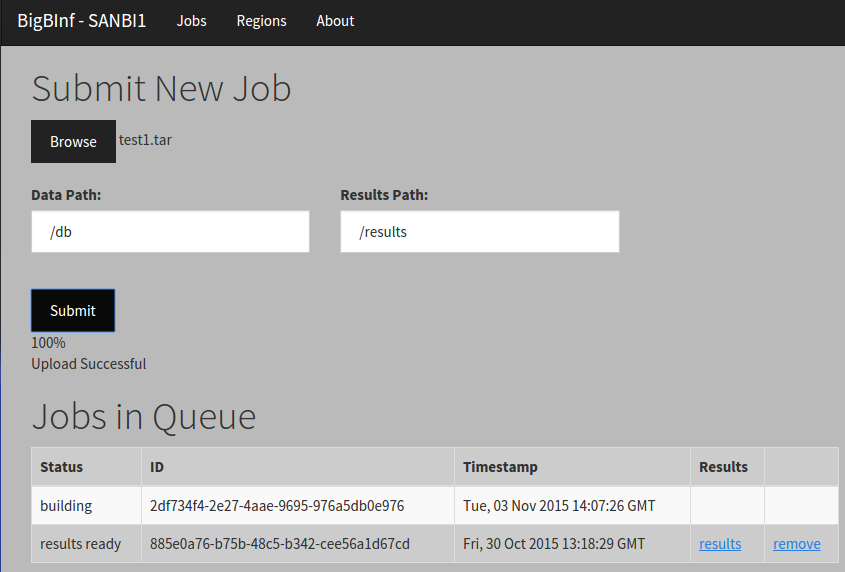
\includegraphics[width=\textwidth]{img/screenshot2.png}
		\caption{The home page which contains a form for submitting a job and a list of jobs currently in the queue}
		\label{fig:screenshot2}
	\end{subfigure}
	\begin{subfigure}[h]{.9\textwidth}
		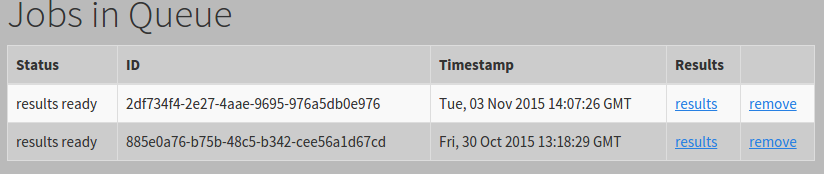
\includegraphics[width=\textwidth]{img/screenshotjobqueue2.png}
		\caption{The job queue after a job is complete}
		\label{fig:screenshotjobqueue}
	\end{subfigure}
	\begin{subfigure}[h]{.5\textwidth}
		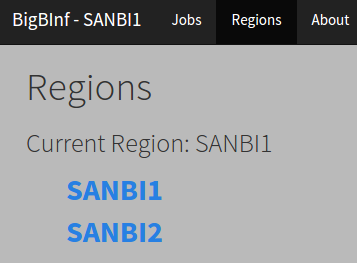
\includegraphics[width=\textwidth]{img/screenshotRegions.png}
		\caption{A list of available micro clouds}
		\label{fig:screenshotRegions}
	\end{subfigure}
\caption{Micro Cloud Screenshots: The frontend web interface available to users. }
\label{fig:screenshots}
\end{figure*}

%\begin{figure*}
%\centering
%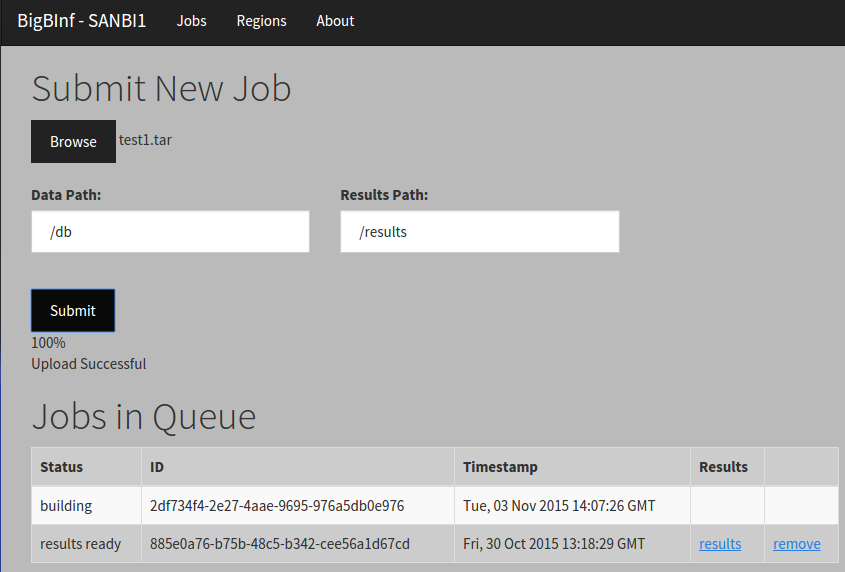
\includegraphics[scale=0.5]{img/screenshot2.png}
%\caption{Micro Cloud Screenshot: The home page.}
%\label{fig:screen1}
%\end{figure*}
%
%\begin{figure*}
%\centering
%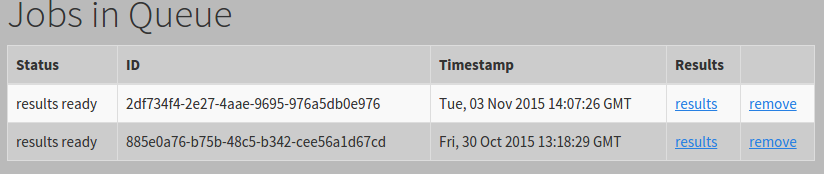
\includegraphics[scale=0.6]{img/screenshotjobqueue2.png}
%\caption{Micro Cloud Screenshot: The job queue after a job is complete.}
%\label{fig:screenjobqueue}
%\end{figure*}
%
%
%\begin{figure*}
%\centering
%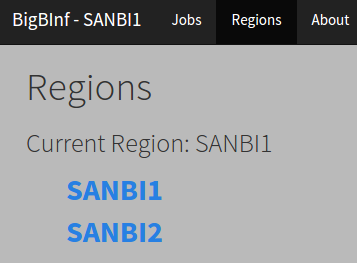
\includegraphics[scale=0.6]{img/screenshotRegions.png}
%\caption{Micro Cloud Screenshot: A list of available micro clouds.}
%\label{fig:screenregions}
%\end{figure*}
\subsection{Image Builder Bottleneck}
Docker saves on storage space and bandwidth with regards to caching docker images. For example if one container uses an Ubuntu base image for the first time, the Ubuntu image must be downloaded. If a second container also uses the same Ubuntu image then it uses the cached copy instead of downloading the image again. This benefit comes from the layered filesystem that Docker uses. 
The base image used in the evaluation is about 600MB in size. This should only have resulted in the first job submitted (which was using that base image) to have a longer build process. The subsequent jobs should have been built in a few seconds. This unfortunately was not the case. Every job took extremely long to move from the build queue to the ready queue. A bottleneck was found after a rigorous investigation. This bottleneck occurs between the Docker builder and the image repository. This means that building the image from the Dockerfile is indeed quick, given that the base image is already cached. The problem occurs when pushing the image to the repository. Docker appears to be pushing the entire image to the repository and spends a lot of time buffering the image to disk, before starting the upload to the repository. Poor performance with pushing a large Docker image seems to be a result of Docker implementation decisions specific to pushing an image to a remote repository. There have been issues opened on this topic on the official Docker Github repository.
\\\\
A change in core architecture of the cluster could fix this bottleneck. The proposed design would be to remove the single dedicated docker builder and instead make every worker node a docker builder. This would mean that the scheduling of building and running jobs would be more tightly integrated, as the image must be built on the worker node that it is scheduled to run on. This would eliminate the need for a private image repository and thus eliminate the process of pushing an image to a repository. Docker is already a dependency for every worker node to be able to run Docker containers. The only problem with this architecture is that it has to be supported by the cluster manager used. In the case of this cloud platform, Kubernetes unfortunately doesn't currently support it. 

\section{Conclusions}
The micro cloud platform implemented is only a proof of concept and requires much more work to be considered ready for deployment. Only the core functionality exists, which is submitting a job that is automatically built and scheduled onto a worker node, and allows downloading the results once the job is complete. It has proved that using Docker containers as a lightweight alternative to virtual machines is a good way to run jobs in an isolated environment, while making the execution environment flexible and user configurable. This is important as it does not restrict a user to a limited set of configured tools, and is thus more maintainable because the administrator is not required to keep the tools up to date. A user configurable environment does not mean that it is time consuming, because Dockerfiles allow re-using a specific environment and simply adding to it the extra requirements. The public Docker repository allows people to share their configured environment created by a Dockerfile. 
\\\\
While Docker allows sharing of configured execution environments, sharing micro cloud deployments between institutions is the real focus. The discovery service creates a loosely coupled community cloud. It allows the user to see a list of the connected micro clouds and choose to redirect to a different micro cloud. This is simple but effective in promoting collaboration between micro clouds.

\subsection{Future Work}
The micro cloud platform provides basic functionality, but entirely neglects aspects such as security. The discovery service needs to be extended to include a central authentication system which allows users from any micro cloud to login and use any other connected micro cloud. Security would also include managing access to raw data. There might be privacy concerns with certain data and more granular access control to specific data would be required to meet security standards.
\\\\
There is also the issue of the docker builder bottleneck. The proposed architecture change discussed in the findings would fix this issue, however implementing this architecture would mean adding core functionality to the Kubernetes framework itself. This would not be an easy task, but would be well worth the effort. It is also possible that the Kubernetes team might add this functionality in the future, as kubernetes is still new and limited in functionality. The alternative would be to test other container manager frameworks to find a cluster manager that is better equipped compared to Kubernetes.

\section{Acknowledgements}
Thanks to Mr. Peter van Heusden and his colleagues (South African National Bioinformatics Institute) for enabling the evaluation of this project by providing two VMs as well as Ceph RBD storage. They were extremely helpful by providing timeous support when problems occurred. In addition, Peter also provided the analysis code used in the evaluation and helped with making the 36GB database available on the RBD storage.
\\
\bibliographystyle{abbrv}
\bibliography{ref} 


\end{document}
